% !TEX root = tracking.tex
\section{Offline Computation \label{sec:precomp}}
The offline computation begins with setting up a capture-avoid game between the tracking system and the planning system, which we then analyze using HJ reachability. In this game, the tracking system will try to ``capture" the planning system, while the planning system is doing everything it can to avoid capture. In reality the planner is typically not actively trying to avoid the tracking system, but this allows us to account for worst-case scenarios. If both systems are acting optimally in this way, we want to determine the largest relative distance that may occur over time. This distance is the maximum possible tracking error between the two systems.

\subsection{Relative Dynamics}
To determine the relative distance that may occur over time we must first define the relative states and dynamics between the tracking and planning models. The individual dynamics are defined in Section \ref{sec:formulation}, equations (\ref{eq:tdyn}) and (\ref{eq:pdyn}). The relative system is found by fixing the planning model to the origin and finding the dynamics of the tracking model relative to the planning model, as shown below.

\begin{equation}
\label{eq:rdyn}
\begin{aligned}
\rstate = \tstate - \ptmat\pstate\\
\dot\rstate = \rdyn(\rstate, \tctrl, \pctrl, \dstb)
\end{aligned}
\end{equation}

Matrix $\ptmat$ matches the common states of $\tstate$ and $\pstate$ by augmenting the state space of the planning model. The relative states $\rstate$ now represent the tracking states relative to the planning states. A similar matrix $\tpmat$ projects the state space of the tracking model onto the planning model: $\pstate = \tpmat(\tstate-\rstate)$. This will be used to update the planning model in the online algorithm.

\subsection{Formalizing the Capture-Avoid Game}
Now that we have the relative dynamics between the two systems we must define a metric for the tracking error bound between these systems. We do this by defining an implicit surface function as a cost function $\errfunc(\rstate)$ in the new frame of reference. Because the metric we care about is distance to the origin (and thus distance to the planner), this cost function can be as simple as distance in position space to the origin. An example can be seen in Fig. \ref{fig:quad4D_example}-a, where $\errfunc(\rstate)$ is defined for a 4D quadrotor model tracking a 2D kinematic planning model. The contour rings beneath the function represent varying level sets of the cost function. The tracking system will try to minimize this cost to reduce the relative distance, while the planning system will do the opposite.
\begin{figure}
	\centering
	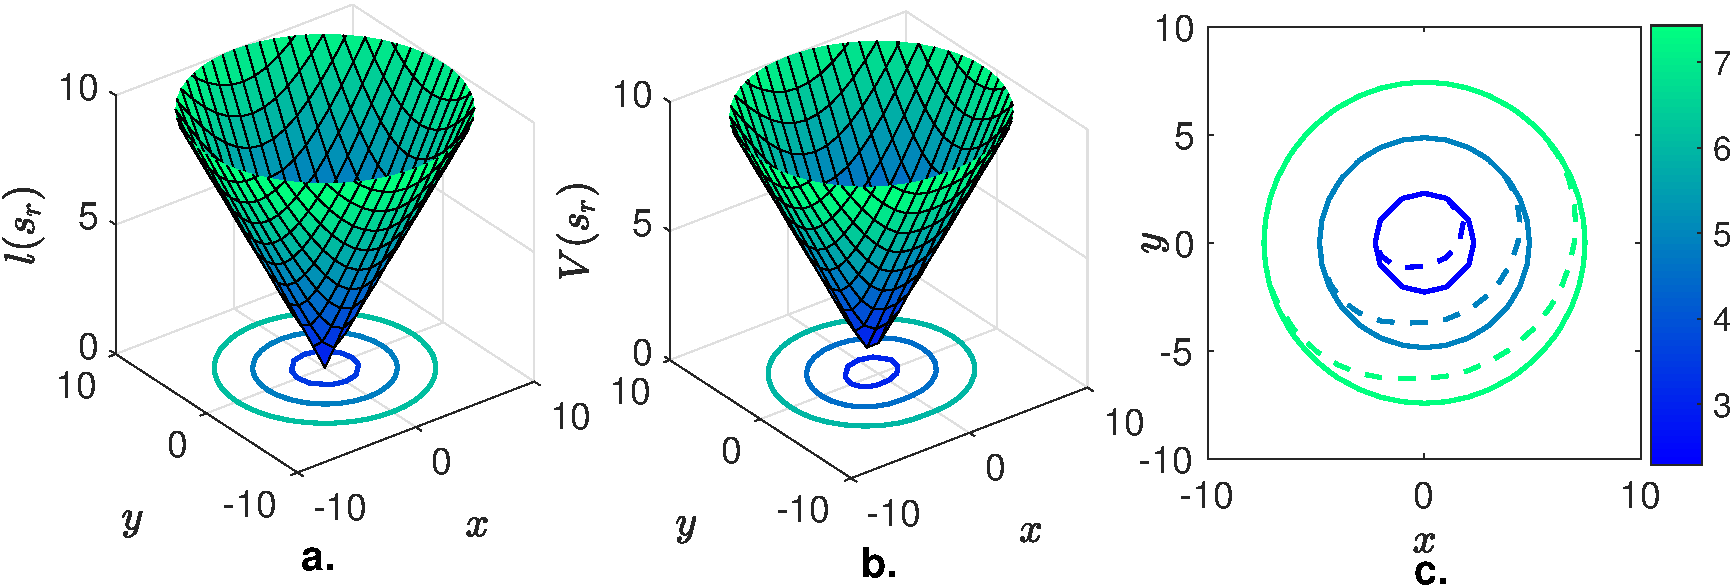
\includegraphics[width=0.5\textwidth]{fig/quad4D_example}
	\caption{illustrative example of the precomputation steps for a 4D quadrotor model tracking a 2D kinematic planning model. All graphs are defined over a 2D slice of the 4D system. a) Cost function $\errfunc(\rstate)$ defined on relative states as distance to the origin, b) Value function $\valfunc(\rstate)$ computed using HJ reachability, c) Level sets of $\errfunc(\rstate)$ (solid) and $\valfunc(\rstate)$ (dashed). If the initial relative state is contained within the dashed set the system is guaranteed to remain within the corresponding solid set (i.e. the tracking error bound)}
	\label{fig:quad4D_example}
	\vspace{-.2in}
\end{figure} 

 We want to find the farthest distance (and thus highest cost) that this game will ever reach when both players are acting optimally. Therefore we want to find a mapping between the initial relative state of the system and the maximum possible cost achieved over the time horizon. This mapping is through our value function, defined as:
 \begin{equation}
 \begin{aligned}
 \label{eq:valfunc}
 	V(\rstate,\thor)= \inf_{\tctrl(\cdot)} \sup_{\pctrl(\cdot), \dstb(\cdot)}  \big\{\max_{\tvar\in [0, \thor]} \errfunc(\rtraj(\tvar; \rstate, 0, \tctrl(\cdot), \pctrl(\cdot)))\big\}
 	\end{aligned}
 \end{equation} 
 This is a modified version of the Hamilton-Jacobi formulation as described by \cite{Fisac15}. By implementing HJ reachability analysis we solve for this value function over the time horizon. If the control authority of the tracking system is powerful enough to always eventually reach the planning system, this value function will converge to an invariant solution for all time, i.e. $\valfunc_\infty(\rstate) := \lim_{\thor\rightarrow\infty} \valfunc(\rstate, \thor)$. An example of this converged value function is in Fig. \ref{fig:quad4D_example}-b. In the next section we will prove that the sub-level sets of this value function will map initial relative states to the guaranteed furthest possible tracking error over all time, as seen in Fig. \ref{fig:quad4D_example}-c.
 
In the context of the online framework, the value function $\valfunc_\infty(\rstate)$ is the tracking error bound function. The spatial gradients of the value function, $\deriv_\infty(\rstate)$, comprise the safety controller function (as describe in Section \ref{sec:online}). When the framework is executed on a computer, these two functions are saved as look-up tables over a grid representing the state space of the relative system.
 
\subsection{Invariance of converged value function}
 \begin{prop}
   \label{prop:main}
   Let suppose that value function converges, and define
      \begin{equation}
      \label{eq:conv_valfunc}
      \valfunc_\infty(\rstate) := \lim_{\thor\rightarrow\infty}\valfunc(\rstate, T)
      \end{equation}
 
   Then $\forall \tvar_1, \tvar_2$ with $\tvar_2 \ge \tvar_1$,
   \begin{equation}
   \label{eq:invariant}
   \valfunc_\infty(\rstate) \ge \valfunc_\infty\Big(\rtraj^*(\tvar_2;, \rstate, \tvar_1)\Big)
   \end{equation}
   \noindent where
   \begin{equation}
   \begin{aligned}
   & \rtraj^*(\tvar;, \rstate, 0) := \rtraj(\tvar; \rstate, 0, \tctrl^*(\cdot), \pctrl^*(\cdot), \dstb^*(\cdot))) \\
   & \tctrl^*(\cdot) = \arg \inf_{\tctrl(\cdot)} \sup_{\pctrl(\cdot), \dstb(\cdot)}\big\{ \\
   & \qquad \max_{\tvar \in [0, \thor]} \errfunc(\rtraj(\tvar; \rstate, 0, \tctrl(\cdot), \pctrl(\cdot), \dstb(\cdot))) \big\}\\
   & \pctrl^*(\cdot) = \arg \sup_{\pctrl(\cdot)} \sup_{\dstb(\cdot)} \big\{ \\
   & \qquad \max_{t \in [0, \thor]} \errfunc(\rtraj(\tvar; \rstate, 0, \tctrl(\cdot), \pctrl(\cdot), \dstb(\cdot))) \big\} \\
   & \dstb^*(\cdot) = \arg \sup_{\dstb(\cdot)} \big\{\max_{\tvar \in [0, \thor]} \errfunc(\rtraj(\tvar; \rstate, 0, \tctrl(\cdot), \pctrl(\cdot),  \dstb(\cdot))) \big\}
   \end{aligned}
   \end{equation}
 \end{prop}

Proposition \ref{prop:main} below proves that every level set of $\valfunc_\infty(\rstate)$ is invariant under the following conditions:
\begin{enumerate}
  \item The tracking system applies the optimal control which tries to track the planning system;
  \item The planning system applies the optimal control that tries to escape from the tracking system; \label{ln:plan}
  \item The tracking system experiences the worst-case disturbance. \label{ln:dist}
\end{enumerate}
In practice, conditions \ref{ln:plan} and \ref{ln:dist} may not hold; the result of this is only advantageous to the tracking system and will make it easier to stay within its current level set of $\valfunc_\infty(\rstate)$, or to move to a smaller invariant level set of $\valfunc_\infty(\rstate)$. The smallest invariant level set $\underline\valfunc := \min_{\rstate} \valfunc_\infty(\rstate)$ can be interpreted as the smallest possible tracking error of the system. The tracking error bound is given by\footnote{In practice, since $\valfunc_\infty$ is obtained numerically, we set $\TEB = \{\rstate: \valfunc_\infty(\rstate) \le \underline\valfunc + \epsilon\}$ for some suitably small $\epsilon>0$} the set $\TEB = \{\rstate: \valfunc_\infty(\rstate) \le \underline\valfunc\}$. This tracking error bound in the planner's frame of reference is given by:
\begin{equation} \label{eq:TEBp}
\TEB_\pstate(\tstate) = \{\pstate: \valfunc_\infty(\tstate-\ptmat\pstate) \le \underline\valfunc\}
\end{equation}
This is the tracking error bound that will be used in the online framework as shown in Fig. \ref{fig:fw_online}. We now prove Proposition \ref{prop:main}.

\begin{proof}
Without loss of generality, assume $\tvar_1=0$. By definition, we have
\begin{equation}
\begin{aligned}
\valfunc_\infty(\rstate) & = \lim_{\thor\rightarrow\infty}\max_{\tvar \in [0, \thor]} \errfunc(\rtraj^*(\tvar; \rstate, 0))\\
\end{aligned}
\end{equation}
By time-invariance, for some $\tvar_2 > 0$,
\begin{equation}
\label{eq:valfunc_ineq}
  \begin{aligned}
\valfunc_\infty(\rstate) &= \lim_{\thor\rightarrow\infty}\max_{\tvar \in [-\tvar_2, \thor]} \errfunc(\rtraj^*(\tvar; \rstate, -\tvar_2)) \\
&\ge \lim_{\thor\rightarrow\infty}\max_{\tvar \in [0, \thor]} \errfunc(\rtraj^*(\tvar; \rstate, -\tvar_2)) 
  \end{aligned}
\end{equation}  
\noindent where the sub-interval $[-\tvar_2, 0)$ has been removed in the last line. Next, by time invariance again, we  have
\begin{equation}
\begin{aligned}
\rtraj^*(\tvar; \rstate, -\tau) &= \rtraj^*(\tvar; \rtraj^*(0; \rstate, -\tvar_2), 0) \\
&= \rtraj^*(\tvar; \rtraj^*(\tvar_2; \rstate, 0), 0)
\end{aligned}
\end{equation}

Now, \eqref{eq:valfunc_ineq} implies

\begin{equation}
\begin{aligned}
\valfunc_\infty(\rstate) &\ge \lim_{\thor\rightarrow\infty}\max_{\tvar \in [0, \thor]} \errfunc(\rtraj^*(\tvar; \rtraj^*(\tvar_2; \rstate, 0), 0)) \\
&= \valfunc_\infty(\rtraj^*(\tvar_2; \rstate, 0))
\end{aligned}
\end{equation} 
\end{proof} 

 
 
 \begin{rem} 
   Proposition \ref{prop:main} is very similar to well-known results in differential game theory with a slightly different cost function \cite{Akametalu2014}, and has been utilized in the context of using the subzero level set of $\valfunc_\infty$ as a backward reachable set for tasks such as collision avoidance or reach-avoid games \cite{Mitchell05}. In our work we do not assign special meaning to any particular level set, and instead consider all level sets at the same time. This effectively allows us to perform solve many simultaneous reachability problems in a single computation, thereby removing the need to check whether resulting invariant sets are empty, as was done in \cite{Bansal2017}.
 \end{rem}